\mysection{Objectif}
L'objectif de ce document est faire un rapport du stage, qui détaille le lieu de travail, toutes les choses produits pendant le stage en expliquant les méthodes utilisés et qui montre les résultats obtenus, les commente et dit les implications des conclusions.
\mysection{Introduction Générale}
Afin de compléter la formation du 2A CentraleSupélec, un stage a été réalisé entre lesm ois de juillet et septembre de 2017, au sein du laboratoire de l'équipe \gls{AUT} du	
\gls{IETR} en travaillant au cadre du projet d'\title, avec la orientation de M. Hervé GUÉGUEN.


\mysubsection{Sur le lieu de travail} 
\mysubsubsection{L'IETR}
L'IETR est un institut de recherche français, spécialisé en électronique et télécommunication, localisé à Rennes, comptant avec plus que 300 enseignants-chercheurs, ingénieurs, doctorants et administratifs, il est formé par équipes de recherche des écoles et instituts de recherche de la région comme le CNRS, l'Université Rennes 1, INSA de Rennes, CentraleSupélec et Université de Nantes.

En relation aux partenariats avec autres instituts et entreprises, L'IETR a une liste considérable de partenaires, incluent des centres publiques comme CEA, CNES et Club Automatique et Automatisation industrielle de la SEE, petites et moyennes entreprises privés comme A\&P Lithos, Adlightec et Advansee, et grandes groupes comme Alstom, EDF et Mitsubishi. 

Son partenariat International compte sur plus de 70 Universités, Instituts et Agences de recherche parmi tout le monde, incluent \gls{JPL}, \gls{Polimi} et \gls{USP}.

\mysubsubsection{Division des Équipes de Recherche}
Afin de meilleur catégoriser les thématiques des projets de recherche L'IETR est divisé en 6 départements/équipes:

\begin{itemize}
	\item Antennes \& Dispositifs Hyperfréquences (ADH)
	\item Signal \& Communications (SC)
	\item Ondes \& Signaux (OS)
	\item Image
	\item Microélectronique \& Microcapteurs (MM)
	\item Automatique (AUT)
\end{itemize}

L'organigramme structurel avec tant les parties de recherche quant les parties administratifs du IETR peut être vu dans la figure \ref{fig:organigramme_IETR_160717_v28}.
\pagebreak

\mysubsubsection{L'équipe AUT}
L'équipe de Automatique est basé a CentraleSupélec et travaille dans diverses thématiques utilisant les connaissances des domaines de analyse et commande des systèmes hybrides.

Ses projets ont des applications que couvrent diverses métiers, on peut voir quelques exemples de projets: comme dans le métier des bâtiments intelligents ( régulation de chauffage pour augmenter l'efficience énergétique )  ,  de la santé ( models des pancréas artificiels pour contrôler le métabolisme de glucose ), du transport ( stratégies de régulation de vitesse des automobiles) , de la distribution d'énergie ( Études de stabilisation de tension de générateurs distribués dans un réseau de distribution ) entre autres.

\vspace{.5cm}
\begin{figure}[H]
	\begin{center}	
		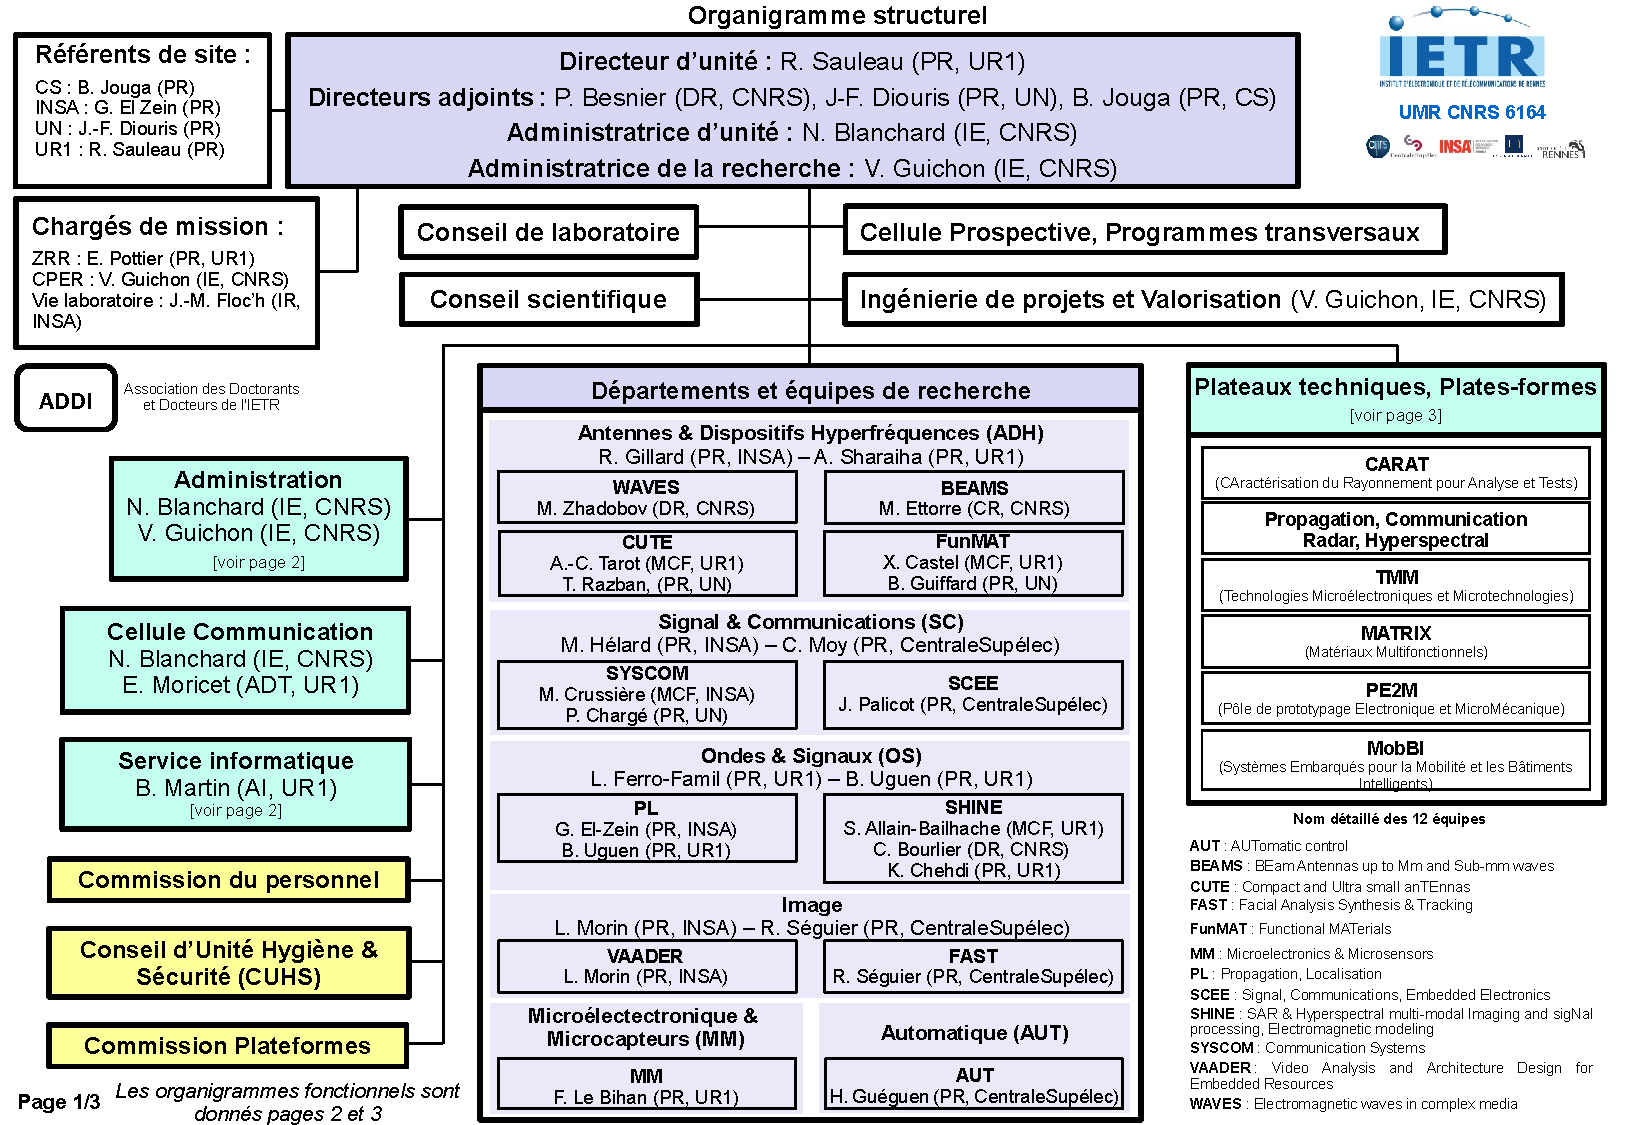
\includegraphics[width=\textwidth]{./organigramme_IETR_160717_v28.pdf}
		\caption{Organigramme du IETR.}
		\label{fig:organigramme_IETR_160717_v28}
	\end{center}
\end{figure}












